\chapter{非理想硬件条件下去蜂窝大规模MIMO系统的URLLC服务资源分配策略}\label{chap:MIMOLP}

在第三章中，本文研究了块长足够长条件下非理想硬件CF-mMIMO系统的可达速率优化问题。然而，工业自动化等物联网关键应用对URLLC提出了毫秒级时延与极高可靠性的严苛需求，短传输块特性使得第三章的长码块假设不再适用。为此，本章聚焦硬件损伤条件下CF-mMIMO系统的URLLC性能优化问题，构建了非线性PA的损伤模型，推导了有限块长下上行链路UE速率闭合表达式。为降低传统优化算法的计算复杂度，提出基于GNN与DRL融合的智能功率控制策略，通过图嵌入技术建模UE空间相关性，动态抑制硬件损伤与时变信道干扰。所提方案在保持毫秒级时延的同时，为工业自动化等物联网应用提供理论与技术支撑。

\section{引言}

随着移动通信技术的不断演进，第五代及未来移动通信网络正推动智能制造、智能交通等物联网应用的快速发展。该网络主要承载超可靠低延迟通信（URLLC）、增强型移动宽带（eMBB）和大规模机器类通信（mMTC）三大核心场景，各场景对可靠性、时延、传输速率及连接密度的服务质量提出了差异化且严苛的要求。其中，URLLC以极端事件响应为目标，要求时延控制在1-10毫秒、误块率低至$10^{-5}$-$10^{-7}$，成为支撑机器人协同控制、自动驾驶等关键任务的核心技术。然而，URLLC的短传输块特性使得传统香农容量理论难以直接适用，现有蜂窝网络架构在保障服务质量方面也面临结构性瓶颈。

去蜂窝大规模多输入多输出（CF-mMIMO）系统作为新一代网络架构，为URLLC服务提供了创新性解决方案。该系统通过分布式部署大量接入点（AP），并与中央处理单元（CPU）协同工作，有效消除蜂窝边缘干扰，实现全域均匀服务覆盖。与传统集中式大规模MIMO相比，CF-mMIMO缩短了AP与UE的空间距离，显著降低信号传播衰落；其稀疏空间布局与多元宏观特征能够稳定信道状态，形成独特的信道硬化效应。这些技术特性为URLLC可靠性提升提供了坚实保障，展现出显著的技术优势。

本章以CF-mMIMO系统的URLLC服务为研究对象，重点探讨硬件损伤条件下的功率分配优化问题。与第三章同时考虑PA非线性与低分辨率ADC的联合影响不同，本章聚焦于UE端非线性PA这一核心硬件损伤因素，通过简化AP端为理想高精度ADC，深入剖析PA非线性对URLLC短包传输性能的内在影响机理。在此基础上，采用无记忆多项式模型刻画PA失真特性，推导有限块长下上行链路用户速率的解析表达式，为后续智能功率控制策略的设计奠定理论基础。

\section{模型设计}

本章在第三章系统模型的基础上进行简化，重点研究仅存在PA非线性硬件损伤的场景。相较于第三章同时考虑PA非线性和低分辨率ADC的复杂模型，本章假设AP端配备理想的高精度ADC（即$b_m \to \infty$，$\alpha_m = 1$），从而能够更加聚焦地分析PA非线性对URLLC服务性能的影响。该简化模型不仅有助于理论推导的清晰性，更能深入揭示硬件损伤与URLLC性能之间的内在关联机制。

\subsection{信道估计}

考虑一个上行链路CF-mMIMO系统，该系统由$M$个配备$N$根天线的AP和$K$个单天线UE构成。第$m$个AP与第$k$个UE之间的信道向量可建模为
\begin{equation}
\mathbf{g}_{mk} = \beta_{mk}^{1/2} \mathbf{h}_{mk},
\end{equation}
其中，$\beta_{mk}$表示大尺度衰落效应，$\mathbf{h}_{mk}$为小尺度衰落向量，其各元素服从独立同分布的复高斯分布$\mathcal{CN}(0,1)$。

为刻画UE端PA的非线性特性，采用无记忆多项式模型进行建模。经非线性PA处理后，第$k$个UE发送的导频信号可表示为
\begin{equation}
\boldsymbol{\phi}_k = \tilde{a}_1\boldsymbol{\varphi}_k + \tilde{a}_3\boldsymbol{\varphi}_k\|\boldsymbol{\varphi}_k\|^2,
\end{equation}
其中，$\tilde{a}_1 = a_1\sqrt{\tau_\text{p}}$，$\tilde{a}_3 = a_3\tau_\text{p}\sqrt{\tau_\text{p}}$，$a_1$和$a_3$分别为无记忆多项式模型的一阶和三阶复系数。

第$m$个AP接收到的导频信号为
\begin{equation}
\mathbf{Y}_{\text{p},m} = \sqrt{\rho_\text{p}}\sum_{k=1}^{K}\mathbf{g}_{mk}\boldsymbol{\phi}_k^H + \mathbf{W}_{\text{p},m},
\end{equation}
其中，$\rho_\text{p}$为导频信号功率，$\mathbf{W}_{\text{p},m}$为加性高斯白噪声矩阵。

鉴于本章假设AP配备理想高精度ADC，即$\alpha_m = 1$且量化噪声可忽略不计，AP可直接对接收信号进行投影处理。将接收信号$\mathbf{Y}_{\text{p},m}$投影至导频序列$\boldsymbol{\varphi}_k$，得到
\begin{equation}
\check{\mathbf{y}}_{\text{p},mk} = \sqrt{\rho_\text{p}}\sum_{k'\in\mathcal{P}_k}(\tilde{a}_1+\tilde{a}_3\tau_\text{p})\mathbf{g}_{mk'} + \mathbf{W}_{\text{p},m}\boldsymbol{\varphi}_k,
\end{equation}
其中，$\mathcal{P}_k$表示与第$k$个UE共享相同导频序列的UE集合。

采用最小均方误差（MMSE）估计算法，信道向量$\mathbf{g}_{mk}$的估计值可表示为
\begin{equation}
\hat{\mathbf{g}}_{mk} = c_{mk}\check{\mathbf{y}}_{\text{p},mk},
\end{equation}
其中，MMSE估计系数$c_{mk}$由下式给出：
\begin{equation}
c_{mk} = \frac{\sqrt{\tau_\text{p}\rho_\text{p}}\beta_{mk}(a_1+a_3\tau_\text{p})}{\tau_\text{p}\rho_\text{p}\sum_{k'\in\mathcal{P}_k}(a_1+a_3\tau_\text{p})^2\beta_{mk'}+1}.
\end{equation}

信道估计向量第$n$个分量的均方值可推导为
\begin{equation}
\gamma_{mk} = \frac{\tau_\text{p}\rho_\text{p}\beta_{mk}^2(a_1+a_3\tau_\text{p})^2}{\tau_\text{p}\rho_\text{p}\sum_{k'\in\mathcal{P}_k}(a_1+a_3\tau_\text{p})^2\beta_{mk'}+1}.
\end{equation}

定义信道估计误差向量为$\tilde{\mathbf{g}}_{mk} = \mathbf{g}_{mk} - \hat{\mathbf{g}}_{mk}$，其各元素服从复高斯分布$\mathcal{CN}(0, \beta_{mk}-\gamma_{mk})$，反映了信道估计的不确定性。

\subsection{上行数据传输}

在上行数据传输阶段，考虑UE端PA的非线性特性。第$k$个UE经非线性PA处理后的输出信号可表示为
\begin{equation}
y_k = \sqrt{\rho_\text{u}}\left(\tilde{a}_{1k}q_k + \tilde{a}_{3k}q_k|q_k|^2\right),
\end{equation}
其中，$\tilde{a}_{1k} = a_1\sqrt{\eta_k}$，$\tilde{a}_{3k} = a_3\eta_k\sqrt{\eta_k}$，$\eta_k$为功率控制系数，需满足功率约束条件$|a_1|^2\eta_k + 2(a_1^*a_3+a_1a_3^*)\eta_k^2 + 6|a_3|^2\eta_k^3 \leq 1$。

第$m$个AP接收到的上行信号为
\begin{equation}
\mathbf{y}_{\text{u},m} = \sqrt{\rho_\text{u}}\sum_{k=1}^{K}\left(\tilde{a}_{1k}\mathbf{g}_{mk}q_k + \tilde{a}_{3k}\mathbf{g}_{mk}q_k|q_k|^2\right) + \mathbf{w}_{\text{u},m},
\end{equation}
其中，$\rho_\text{u}$为上行数据传输功率，$\mathbf{w}_{\text{u},m} \sim \mathcal{CN}(\mathbf{0},\mathbf{I}_N)$为加性高斯白噪声。

在CPU处，采用MF接收信号进行处理，第$k$个用户的合并信号为
\begin{equation}
r_{\text{u},k} = \sum_{m=1}^{M}\hat{\mathbf{g}}_{mk}^H\mathbf{y}_{\text{u},m}.
\end{equation}

\subsection{可达速率分析}

为分析系统性能，将接收信号$r_{\text{u},k}$分解为多个分量：
\begin{equation}
r_{\text{u},k} = \text{ES}_k \cdot q_k + \text{BU}_k \cdot q_k + \sum_{k'\neq k}^{K}\text{I}_{kk'} \cdot q_{k'} + \sum_{k'\neq k}^{K}\text{NB}_{kk'} \cdot q_{k'} + \text{N}_k,
\end{equation}
其中，各分量分别表示期望信号（ES）、波束成形增益不确定性（BU）、用户间干扰（I）、非线性干扰（NB）以及加性噪声（N）。

基于信道估计误差模型$\mathbf{g}_{mk} = \hat{\mathbf{g}}_{mk} + \tilde{\mathbf{g}}_{mk}$及MMSE估计的统计特性，期望信号分量可推导为
\begin{equation}
\text{ES}_k = N\sqrt{\rho_\text{u}}(\tilde{a}_{1k}+\tilde{a}_{3k})\sum_{m=1}^{M}\gamma_{mk}.
\end{equation}

加性噪声分量的方差为
\begin{equation}
\mathbb{E}\{|\text{N}_k|^2\} = N\sum_{m=1}^{M}\gamma_{mk}.
\end{equation}

假设总干扰$\Theta_k$包含波束成形增益不确定性、UE间干扰和PA非线性损伤三个主要部分。其方差可简化为如下表达式：
\begin{equation}
\mathbb{E}\{|\Theta_k|^2\} = N\rho_\text{u}\sum_{k'=1}^{K}\Omega_{k'}\sum_{m=1}^{M}\gamma_{mk}\beta_{mk'} + 3N\rho_\text{u}|a_3|^2\eta_k^3\left(\sum_{m=1}^{M}\gamma_{mk}\right)^2,
\end{equation}
其中，$\Omega_k = |a_1|^2\eta_k + 2(a_1^*a_3+a_1a_3^*)\eta_k^2 + 6|a_3|^2\eta_k^3$表征第$k$个UE的有效发射功率。

\subsection{上行可达速率闭合表达式}

基于前述分析结果，第$k$个UE的上行可达速率可表示为
\begin{equation}
R_{\text{u},k} = \log_2\left(1 + \text{SINR}_k\right),
\end{equation}
其中，$\text{SINR}_k$的闭合表达式为
\begin{equation}\label{SINR}
\text{SINR}_k = \frac{N\rho_\text{u}|\tilde{a}_{1k}+\tilde{a}_{3k}|^2\left(\sum_{m=1}^{M}\gamma_{mk}\right)^2}{\rho_\text{u}\sum_{k'=1}^{K}\Omega_{k'}\sum_{m=1}^{M}\gamma_{mk}\beta_{mk'} + 3\rho_\text{u}|a_3|^2\eta_k^3\left(\sum_{m=1}^{M}\gamma_{mk}\right)^2 + \sum_{m=1}^{M}\gamma_{mk}}.
\end{equation}

上述闭合表达式从理论上刻画了PA非线性对系统性能的内在影响机制。具体而言，分子项$|\tilde{a}_{1k}+\tilde{a}_{3k}|^2$量化了PA非线性导致的期望信号功率衰减程度；分母中的$3\rho_\text{u}|a_3|^2\eta_k^3(\sum_{m}\gamma_{mk})^2$项则表征了PA非线性引入的自干扰分量对有效信干噪比的劣化作用。值得注意的是，当$a_3 = 0$时，即理想线性PA条件下，该表达式可退化为经典大规模MIMO系统的性能分析结果，验证了推导的正确性。

相较于第三章式(3-23)所给出的联合硬件损伤模型，本章表达式通过剔除ADC相关的量化噪声项$\Psi_k$及量化系数$\alpha_m$，聚焦于硬件损伤对URLLC场景的影响，更重要的是为后续URLLC性能分析与功率控制算法设计提供了更为聚焦的理论基础，便于深入揭示PA非线性在短包传输场景下的独特影响规律。

\section{可实现URLLC速率}
传统的香农容量是在假设码字长度趋于无穷大、解码错误概率趋近于零的理想条件下推导的。然而，在URLLC场景下，由于对时延和可靠性的极高要求，实际通信往往采用有限块长编码，此时香农容量理论已不再适用。为准确刻画有限块长下的系统性能，URLLC通常采用有限块长编码理论对可实现速率进行分析。

URLLC服务的核心性能评估指标主要涵盖可靠性与时延两个关键维度。可靠性指标采用误块率（Block Error Rate, BLER）$\varepsilon_k$进行量化，该参数表征传输数据包在解码过程中发生错误的概率。基于有限块长信息论的理论框架，第$k$个用户设备的误块率可近似表达为
\begin{equation}
\varepsilon_k \approx Q\left(\frac{nC_k - L_k}{\sqrt{nV_k}}\right),
\end{equation}
式中$n$表示传输块长参数，$L_k$为传输比特数量，$C_k = \log_2(1 + \text{SINR}_k)$为信道容量函数，$V_k = (\log_2 e)^2(1 - (1 + \text{SINR}_k)^{-2})$为信道色散参数。该数学表达式清晰揭示了误块率与信干噪比、传输块长之间的内在关联机制：当信道条件恶化或功率配置不足时，$\text{SINR}_k$的降低将导致信道容量$C_k$相应减小，从而引起误块率的升高。

依据3GPP TS 38.913技术标准规范，URLLC典型应用场景要求误块率不超过$10^{-5}$量级。本文假设所有用户设备采用统一的目标误块率设定值$\varepsilon_k = \varepsilon_{\text{th}} = 10^{-5}$，并基于此参数配置推导可实现速率的闭合表达式。

端到端传输时延$D_k$包含传输时延、处理时延以及排队时延等多个组成部分。本文研究重点聚焦于传输时延的分析，该时延分量由信道相干时间与系统带宽共同决定。具体而言，传输块长$n$满足以下关系式
\begin{equation}
n = \tau_{\text{c}} \cdot W,
\end{equation}
其中,$\tau_{\text{c}}$表示信道相干时间参数，$W$为系统带宽。根据3GPP标准规范，URLLC典型应用要求端到端时延不超过$1$毫秒，本文据此设定时延阈值$D_{\text{th}} = 1$ ms。

基于上述误块率模型与时延约束条件，根据有限块长信息论的理论基础\cite{polyanskiy2010channel}，第$k$个用户设备的URLLC可实现速率可近似表示为：
\begin{equation}
r_{\text{u},k} \approx C_k - \sqrt{\frac{V_k}{n}} Q^{-1}(\varepsilon_{\text{th}}),
\end{equation}
其中$Q^{-1}(\cdot)$为高斯$Q$函数的反函数。该近似表达式在传输块长$n \geq 100$信道使用条件下具有较高的计算精度，适用于URLLC短包传输场景的性能分析。

上述数学表达式系统揭示了URLLC可实现速率与误块率、时延约束之间的内在关联规律：一方面，目标误块率$\varepsilon_{\text{th}}$通过$Q^{-1}(\cdot)$函数直接影响速率修正项的大小，更严格的可靠性要求将导致更大的速率性能损失；另一方面，时延约束$D_{\text{th}}$通过决定传输块长$n$的取值，进而影响信道色散与速率修正幅度。需要特别指出的是，功率放大器非线性损伤会进一步劣化有效信干噪比性能，从而在有限块长传输条件下加剧速率损失效应。该表达式综合考虑了有限块长下的误码概率约束、时延约束以及非理想硬件损伤影响，更加贴合URLLC实际应用场景的技术要求，为后续资源分配算法设计与系统性能优化提供了坚实的理论基础。

\section{上行和速率最大化}
基于上述分析，本节建立非理想硬件条件下CF-mMIMO系统URLLC服务的功率控制优化问题。以最大化系统总可实现速率为目标，同时满足URLLC时延与可靠性约束，优化问题可表述为
\begin{align}
\max_{\boldsymbol{\eta}} \quad & \sum_{k=1}^{K} r_{\text{u},k}(\eta_k) \\
\text{s.t.} \quad & 0 \leq \eta_k \leq \eta_{\max}, \quad \forall k \in \mathcal{K}, \label{constraint:power} \\
& \varepsilon_k \leq \varepsilon_{\max}, \quad \forall k \in \mathcal{K}, \label{constraint:reliability} \\
& D_k \leq D_{\text{th}}, \quad \forall k \in \mathcal{K}, \label{constraint:delay}
\end{align}
其中，$\boldsymbol{\eta} = [\eta_1, \eta_2, \ldots, \eta_K]^T$表示功率控制向量，$r_{\text{u},k}(\eta_k)$的具体表达式由式(4-12)给出。约束条件\eqref{constraint:power}限制各UE的发射功率在$[0, \eta_{\max}]$区间范围内；约束条件\eqref{constraint:reliability}要求误块率不超过最大允许值$\varepsilon_{\max}$，确保满足URLLC服务的可靠性需求；约束条件\eqref{constraint:delay}则保证第$k$个用户设备的端到端时延$D_k$不超过预设阈值$D_{\text{th}}$，其中$D_k$由传输时延、处理时延以及排队时延共同构成。

该优化问题的求解过程面临多重技术挑战：首先，目标函数$r_{\text{u},k}$关于功率变量$\eta_k$呈现非凸特性，且涉及有限块长修正项的复杂非线性运算；其次，功率放大器非线性引入的自干扰效应使得各用户设备速率之间产生相互耦合，形成复杂的干扰拓扑结构；此外，信道状态的时变性要求算法具备实时决策能力，传统集中式优化方法难以满足毫秒级时延的严格要求。针对上述挑战，下一节将提出基于图神经网络与深度强化学习融合的智能功率控制算法，通过分布式学习机制与干扰图建模技术实现优化问题的高效求解。

\section{算法设计}
本小节提出一种基于图神经网络的动态干扰管理算法。该算法通过图神经网络基于信道特征动态提取UE之间的干扰来辅助DRL算法预测，实现多用户干扰关系的自适应建模与功率控制的联合优化。
\subsection{用户节点特征建模}
为了精确建模UE之间的空间分布以及干扰特性，将每个UE定义为图中的节点。考虑到信道状态信息包含幅度和相位两种物理意义明确的特征，本文分别对幅度和相位进行独立建模与融合处理，以充分挖掘信道信息的表征能力。

首先，定义UE $k$到所有AP的聚合信道向量。根据第三章系统模型，第$m$个AP与第$k$个UE之间的信道向量为$\mathbf{g}_{mk} \in \mathbb{C}^{N \times 1}$，其中$N$为每个AP的天线数。将UE $k$到所有$M$个AP的信道向量进行聚合，得到聚合信道向量：
\begin{equation}
\mathbf{g}_{k} = \left[\mathbf{g}_{1k}^{T}, \mathbf{g}_{2k}^{T}, \ldots, \mathbf{g}_{Mk}^{T}\right]^{T} \in \mathbb{C}^{MN \times 1}
\end{equation}

对聚合信道向量$\mathbf{g}_{k}$进行幅度-相位分解：
\begin{equation}
\mathbf{g}_{k} = \mathbf{A}_{k} \odot \exp(j\boldsymbol{\Phi}_{k})
\end{equation}
其中，$\mathbf{A}_{k} = |\mathbf{g}_{k}|$表示信道幅度向量，$\boldsymbol{\Phi}_{k} = \angle\mathbf{g}_{k}$表示信道相位向量，$\odot$表示逐元素乘法。

基于此分解，节点特征采用双分支结构进行编码。幅度分支特征$\mathbf{f}_{k}^{\text{amp}}$捕获信号强度与硬件损伤信息：
\begin{equation}
\mathbf{f}_{k}^{\text{amp}}=\left[\mathbf{A}_{k}^{(1)}, \mathbf{A}_{k}^{(2)}, \ldots, \mathbf{A}_{k}^{(M)}, \eta_{k},\left|a_{3 k}\right|\right]^{T}
\end{equation}
其中，$\mathbf{A}_{k}^{(m)} = |\mathbf{g}_{mk}|$表示用户$k$到第$m$个AP的信道幅度向量，$\eta_{k}$表示当前发射功率，$\left|a_{3 k}\right|$量化了PA非线性失真程度。

相位分支特征$\mathbf{f}_{k}^{\text{ph}}$编码信道方向性与空间相关性：
\begin{equation}
\mathbf{f}_{k}^{\text{ph}}=\left[\boldsymbol{\Phi}_{k}^{(1)}, \boldsymbol{\Phi}_{k}^{(2)}, \ldots, \boldsymbol{\Phi}_{k}^{(M)}, \cos(\theta_{k}), \sin(\theta_{k}), \right]^{T}
\end{equation}
其中，$\boldsymbol{\Phi}_{k}^{(m)} = \angle\mathbf{g}_{mk}$表示UE $k$到第$m$个AP的信道相位向量，$\theta_{k}$为UE $k$的空间方位角。

最终，节点特征通过特征融合层进行整合。首先，幅度分支和相位分支分别经多层感知机映射到统一维度的特征空间：
\begin{equation}
\mathbf{h}_{k}^{\text{amp}} = \mathbf{W}_{\text{amp}}^{(2)} \sigma\left(\mathbf{W}_{\text{amp}}^{(1)} \mathbf{f}_{k}^{\text{amp}} + \mathbf{b}_{\text{amp}}^{(1)}\right) + \mathbf{b}_{\text{amp}}^{(2)}
\end{equation}
\begin{equation}
\mathbf{h}_{k}^{\text{ph}} = \mathbf{W}_{\text{ph}}^{(2)} \sigma\left(\mathbf{W}_{\text{ph}}^{(1)} \mathbf{f}_{k}^{\text{ph}} + \mathbf{b}_{\text{ph}}^{(1)}\right) + \mathbf{b}_{\text{ph}}^{(2)}
\end{equation}
其中，$\mathbf{W}_{\text{amp}}^{(1)}, \mathbf{W}_{\text{amp}}^{(2)}$和$\mathbf{W}_{\text{ph}}^{(1)}, \mathbf{W}_{\text{ph}}^{(2)}$分别为两个分支MLP的权重矩阵，$\mathbf{b}$为偏置向量，$\sigma(\cdot)$为ReLU激活函数。

然后，通过拼接与投影操作实现双分支信息融合：
\begin{equation}
\mathbf{f}_{k} = \mathbf{W}_{\text{fuse}} \left[\mathbf{h}_{k}^{\text{amp}} \| \mathbf{h}_{k}^{\text{ph}}\right] + \mathbf{b}_{\text{fuse}}
\end{equation}
其中，$\|$表示向量拼接操作，$\mathbf{W}_{\text{fuse}} \in \mathbb{R}^{D \times 2D}$为融合投影矩阵，$D$为节点特征的最终维度。

\subsection{干扰边特征建模}
为准确刻画UE间的干扰耦合关系，在图结构中引入边特征建模。对于任意UE节点对$(i, k)$，其边特征$\mathbf{e}_{ik}$定义为：
\begin{equation}
\mathbf{e}_{ik} = \left[d_{ik}, I_{ik}\right]^{T}
\end{equation}
其中，$d_{ik}$表示UE $i$与UE $k$之间的归一化距离，定义为$d_{ik} = \|\mathbf{x}_{i} - \mathbf{x}_{k}\| / d_{\max}$，$\mathbf{x}_{i}$和$\mathbf{x}_{k}$分别为UE $i$和UE $k$的位置坐标，$d_{\max}$为系统覆盖区域的最大距离。该特征用于表征UE间的空间邻近程度，距离越近则潜在干扰越强。$I_{ik}$表示UE间的干扰强度，定义为：
\begin{equation}
I_{ik} = \frac{\|\mathbf{g}_{i}^{H}\mathbf{g}_{k}\|_{F}^{2}}{MN}
\end{equation}
其中，$\|\cdot\|_{F}$表示Frobenius范数。该指标量化了UE间的信道相关性，取值越大表示干扰越强。

边的存在性由干扰阈值判定：
\begin{equation}
\mathcal{E}_{ik} = \begin{cases}
1, & \text{if } I_{ik} > \epsilon_{\text{th}} \\
0, & \text{otherwise}
\end{cases}
\end{equation}
其中$\epsilon_{\text{th}}$为干扰强度阈值，典型设置为$\epsilon_{\text{th}}=0.1$。该稀疏化策略有效降低图结构复杂度，聚焦于关键干扰链路。



\subsection{图神经网络消息传递机制}
基于构建的节点特征和边特征，采用图注意力网络（GAT）实现消息传递与特征聚合。GAT的核心思想是通过注意力机制自适应地学习邻居节点的重要性权重，从而实现差异化信息聚合。

在第$l$层消息传递中，节点$k$首先通过线性变换将其特征映射到新的特征空间：
\begin{equation}
\mathbf{h}_{k}^{\prime(l)} = \mathbf{W}^{(l)}\mathbf{h}_{k}^{(l)}
\end{equation}
其中，$\mathbf{h}_{k}^{(l)}$为节点$k$在第$l$层的隐藏状态（$\mathbf{h}_{k}^{(0)} = \mathbf{f}_{k}$），$\mathbf{W}^{(l)} \in \mathbb{R}^{D \times D}$为可学习的权重矩阵。

然后，计算节点$k$与邻居节点$i$之间的注意力系数。为充分利用边特征信息，采用边增强的注意力机制：
\begin{equation}
e_{ik}^{(l)} = \text{LeakyReLU}\left(\mathbf{a}^{(l)T}\left[\mathbf{h}_{i}^{\prime(l)} \| \mathbf{h}_{k}^{\prime(l)} \| \mathbf{W}_{e}^{(l)}\mathbf{e}_{ik}\right]\right)
\end{equation}
其中，$\|$表示向量拼接操作，$\mathbf{a}^{(l)}$为注意力向量，$\mathbf{W}_{e}^{(l)}$为边特征变换矩阵。该设计将节点特征与边特征联合建模，使注意力系数能够感知用户间的干扰强度。

注意力系数通过softmax函数归一化：
\begin{equation}
\alpha_{ik}^{(l)} = \frac{\exp(e_{ik}^{(l)})}{\sum_{j \in \mathcal{N}(k) \cup \{k\}}\exp(e_{jk}^{(l)})}
\end{equation}
其中，$\mathcal{N}(k)$为节点$k$的邻居节点集合，自环的引入使节点能够保留自身特征信息。

为增强模型的表达能力，采用多头注意力机制。设$H$为注意力头数，各头独立计算注意力系数并进行特征聚合：
\begin{equation}
\mathbf{h}_{k}^{(l+1)} = \sigma\left(\frac{1}{H}\sum_{h=1}^{H}\sum_{i \in \mathcal{N}(k) \cup \{k\}} \alpha_{ik}^{(l,h)} \mathbf{W}^{(l,h)}\mathbf{h}_{i}^{(l)}\right)
\end{equation}
其中，$\alpha_{ik}^{(l,h)}$和$\mathbf{W}^{(l,h)}$分别为第$h$个注意力头的注意力系数和权重矩阵，$\sigma(\cdot)$为ReLU激活函数。多头机制使模型能够从不同子空间捕获节点间的关联特征。

经过$L$层消息传递后，得到各节点的图嵌入表示$\mathbf{z}_{k} = \mathbf{h}_{k}^{(L)}$，该嵌入融合了局部拓扑结构、信道状态及干扰关系信息，为后续功率控制决策提供高维表征。

\subsection{基于Actor-Critic的功率控制决策}
基于GNN提取的图嵌入表示，将功率控制问题建模为马尔可夫决策过程（MDP），采用近端策略优化（PPO）算法进行求解。MDP由状态空间$\mathcal{S}$、动作空间$\mathcal{A}$、状态转移概率$\mathcal{P}$和奖励函数$\mathcal{R}$四元组定义。

系统状态由各用户的图嵌入向量与全局上下文特征组成。对于时隙$t$，状态定义为：
\begin{equation}
\mathbf{s}_{t} = \left[\mathbf{z}_{1}^{(t)}, \mathbf{z}_{2}^{(t)}, \ldots, \mathbf{z}_{K}^{(t)}, \mathbf{c}^{(t)}\right]
\end{equation}
其中，$\mathbf{z}_{k}^{(t)} \in \mathbb{R}^{D}$为用户$k$在时隙$t$经GNN提取的图嵌入，融合了信道状态、干扰关系及拓扑结构信息；$\mathbf{c}^{(t)} = \left[\bar{r}^{(t)}, \bar{\eta}^{(t)}, \bar{I}^{(t)}\right]$为全局上下文特征，分别表示系统平均速率、平均发射功率和平均干扰强度。

动作空间定义为各用户发射功率的调整系数：
\begin{equation}
\mathbf{a}_{t} = \left[\delta_{1}^{(t)}, \delta_{2}^{(t)}, \ldots, \delta_{K}^{(t)}\right], \quad \delta_{k}^{(t)} \in [0, 1]
\end{equation}
实际发射功率为$\eta_{k}^{(t)} = \delta_{k}^{(t)} \cdot \eta_{\max}$，其中$\eta_{\max}$为最大发射功率约束。

Actor网络负责输出功率控制策略。对于用户$k$，其策略均值由图嵌入经全连接层变换得到：
\begin{equation}
\mu_{k}^{(t)} = \mathbf{W}_{\mu}^{(2)} \sigma\left(\mathbf{W}_{\mu}^{(1)} \mathbf{z}_{k}^{(t)} + \mathbf{b}_{\mu}^{(1)}\right) + \mathbf{b}_{\mu}^{(2)}
\end{equation}
其中，$\mathbf{W}_{\mu}^{(1)} \in \mathbb{R}^{D_{\mu} \times D}$和$\mathbf{W}_{\mu}^{(2)} \in \mathbb{R}^{1 \times D_{\mu}}$为可学习权重矩阵，$D_{\mu}$为隐藏层维度。策略分布采用高斯分布建模：
\begin{equation}
\pi_{\theta}(\mathbf{a}_{t}|\mathbf{s}_{t}) = \prod_{k=1}^{K} \mathcal{N}\left(\delta_{k}; \mu_{k}^{(t)}, \sigma^{2}\right)
\end{equation}
其中，标准差$\sigma$为可学习参数，控制探索程度。

Critic网络评估当前状态的期望累积奖励。首先对所有用户的图嵌入进行全局平均池化：
\begin{equation}
\bar{\mathbf{z}}^{(t)} = \frac{1}{K}\sum_{k=1}^{K}\mathbf{z}_{k}^{(t)}
\end{equation}
然后，将池化后的嵌入与全局上下文特征拼接，经多层感知机输出状态值：
\begin{equation}
V_{\phi}(\mathbf{s}_{t}) = \mathbf{W}_{v}^{(2)} \sigma\left(\mathbf{W}_{v}^{(1)} \left[\bar{\mathbf{z}}^{(t)} \| \mathbf{c}^{(t)}\right] + \mathbf{b}_{v}^{(1)}\right) + \mathbf{b}_{v}^{(2)}
\end{equation}
其中，$\mathbf{W}_{v}^{(1)} \in \mathbb{R}^{D_{v} \times (D+3)}$和$\mathbf{W}_{v}^{(2)} \in \mathbb{R}^{1 \times D_{v}}$为可学习权重矩阵。该设计通过聚合全局信息，评估当前功率配置的系统级价值。

\begin{figure}[t]
\centering
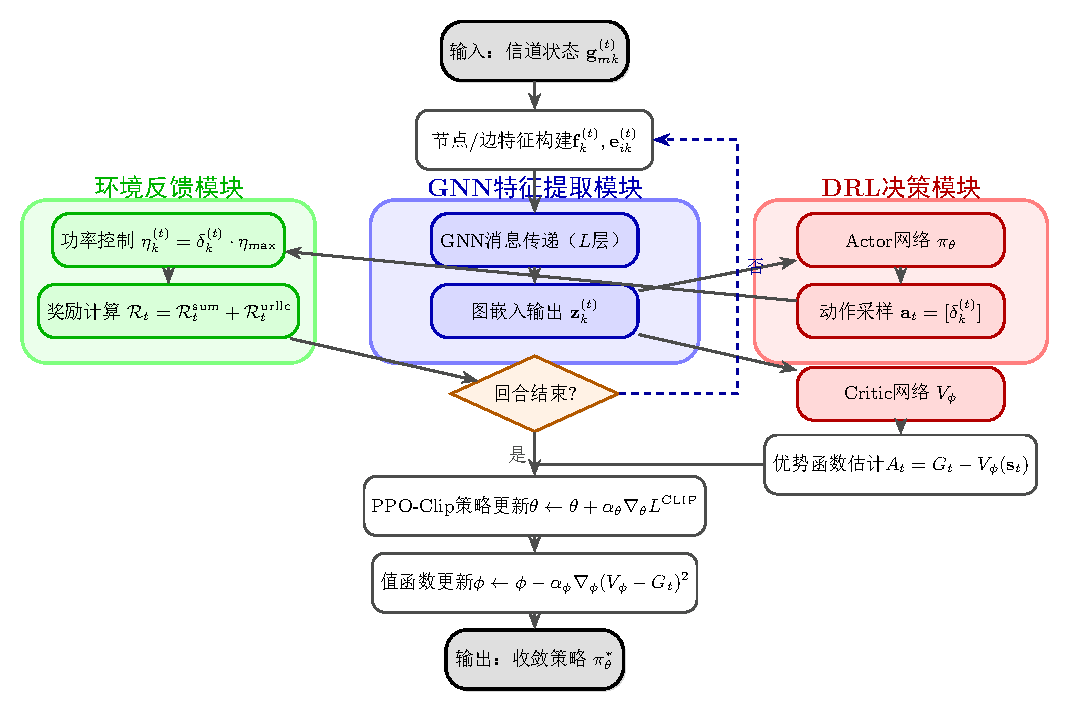
\includegraphics[width=0.95\textwidth]{algorithm_flowchart.pdf}
\caption{基于GNN-DRL的CF-mMIMO功率控制算法流程图}
\label{fig:algorithm_flowchart}
\end{figure}

\subsection{奖励函数设计}
针对CF-mMIMO系统中URLLC功率控制问题，奖励函数综合考虑系统频谱效率及URLLC服务质量约束。本文设计的奖励函数由系统和速率及URLLC约束惩罚构成，各分量分别对应不同的优化目标。

系统和速率作为无线通信系统的核心性能指标，直接表征系统容量与频谱利用效率。对于时隙$t$，系统和速率项定义为：
\begin{equation}
\mathcal{R}_{t}^{\text{sum}} = \frac{1}{K} \sum_{k=1}^{K} r_{\text{u},k}^{(t)}
\end{equation}
其中，$r_{\text{u},k}^{(t)}$表示用户设备$k$在时隙$t$的URLLC可实现速率。通过除以用户总数$K$进行归一化处理，使得系统和速率项在数值量级上与惩罚项相匹配。该奖励项设计旨在引导智能体探索能够最大化系统和容量的功率分配策略。

URLLC应用场景对通信可靠性与传输时延具有极为严格的技术要求，约束条件的违反将导致工业控制、远程医疗等关键应用场景的严重故障。本文采用惩罚函数机制来确保服务质量约束的满足：
\begin{equation}
\mathcal{R}_{t}^{\text{urllc}} = -\lambda_{\varepsilon} \sum_{k=1}^{K} \mathbf{1}_{\left\{\varepsilon_{k}^{(t)} > \varepsilon_{\text{th}}\right\}} - \lambda_{\tau} \sum_{k=1}^{K} \mathbf{1}_{\left\{D_{k}^{(t)} > D_{\text{th}}\right\}}
\end{equation}
其中，$\varepsilon_{k}^{(t)}$和$D_{k}^{(t)}$分别表示用户设备$k$在时隙$t$的解码错误概率与端到端时延；$\varepsilon_{\text{th}}$和$D_{\text{th}}$为URLLC约束阈值参数，依据3GPP TS 38.913技术标准规范，典型值分别设定为$\varepsilon_{\text{th}}=10^{-5}$和$D_{\text{th}}=1$毫秒；$\lambda_{\varepsilon}$和$\lambda_{\tau}$为相应的惩罚系数。

当信道条件恶化或功率配置不足时，解码错误概率升高将触发惩罚机制，从而引导智能体调整功率控制策略以满足可靠性要求。端到端时延$D_{k}^{(t)}$由传输时延、处理时延与排队时延共同构成，在URLLC应用场景下需要严格约束在预设阈值范围内。

综合上述设计要素，总奖励函数的数学表达式为：
\begin{equation}
\mathcal{R}_{t} = \mathcal{R}_{t}^{\text{sum}} + \mathcal{R}_{t}^{\text{urllc}}
\end{equation}
该设计将归一化处理后的系统和速率与URLLC约束惩罚项直接相加。通过对系统和速率项除以用户总数$K$进行归一化，确保了两个组成部分在数值量级上具有可比性，避免单一优化目标主导梯度更新过程，从而使得智能体能够同时优化系统容量性能与URLLC服务质量要求。

\begin{algorithm}[h]
\caption{基于GNN-DRL的CF-mMIMO功率控制算法}
\label{alg:gnn-drl}
\begin{algorithmic}[1]
\Require 训练回合数$N_{\text{ep}}$，每回合时隙数$T$，Actor学习率$\alpha_{\theta}$，Critic学习率$\alpha_{\phi}$，折扣因子$\gamma$，PPO裁剪参数$\epsilon$
\Ensure 收敛的策略网络参数$\theta$与值网络参数$\phi$
\State 随机初始化GNN参数$\Theta_{\text{GNN}}$，Actor参数$\theta$，Critic参数$\phi$
\For{$n = 1$ \textbf{to} $N_{\text{ep}}$}
    \For{$t = 1$ \textbf{to} $T$}
        \State 基于信道状态构建节点特征$\{\mathbf{f}_{k}^{(t)}\}_{k=1}^{K}$与边特征$\{\mathbf{e}_{ik}^{(t)}\}$
        \State 执行$L$层GNN消息传递，输出图嵌入$\mathbf{z}_{k}^{(t)} = \text{GNN}(\mathbf{f}_{k}^{(t)}, \{\mathbf{e}_{ik}^{(t)}\})$
        \State 构建系统状态$\mathbf{s}_{t} = [\mathbf{z}_{1}^{(t)}, \ldots, \mathbf{z}_{K}^{(t)}, \mathbf{c}^{(t)}]$，Actor采样动作$\mathbf{a}_{t} \sim \pi_{\theta}(\cdot|\mathbf{s}_{t})$
        \State 执行功率控制$\eta_{k}^{(t)} = \delta_{k}^{(t)} \cdot \eta_{\max}$，计算归一化系统和速率$\mathcal{R}_{t}^{\text{sum}} = \frac{1}{K}\sum_{k=1}^{K}r_{\text{u},k}^{(t)}$与URLLC惩罚$\mathcal{R}_{t}^{\text{urllc}}$
        \State 观测即时奖励$\mathcal{R}_{t} = \mathcal{R}_{t}^{\text{sum}} + \mathcal{R}_{t}^{\text{urllc}}$
        \State 存储转移样本$(\mathbf{s}_{t}, \mathbf{a}_{t}, \mathcal{R}_{t}, \mathbf{s}_{t+1})$至经验回放池$\mathcal{D}$
    \EndFor
    \State 从$\mathcal{D}$随机采样批量样本，计算折扣累积奖励$G_{t} = \sum_{l=0}^{\infty}\gamma^{l}\mathcal{R}_{t+l}$
    \State 估计优势函数$A_{t} = G_{t} - V_{\phi}(\mathbf{s}_{t})$，计算PPO-Clip目标函数$L^{\text{CLIP}}(\theta)$
    \State 梯度上升更新Actor：$\theta \leftarrow \theta + \alpha_{\theta}\nabla_{\theta}L^{\text{CLIP}}(\theta)$
    \State 梯度下降更新Critic：$\phi \leftarrow \phi - \alpha_{\phi}\nabla_{\phi}(V_{\phi}(\mathbf{s}_{t})-G_{t})^{2}$
    \State 反向传播端到端联合优化GNN参数$\Theta_{\text{GNN}}$
\EndFor
\end{algorithmic}
\end{algorithm}

\subsection{算法训练流程}

本文提出的GNN-DRL融合算法的整体架构框架如图\ref{fig:algorithm_flowchart}所示。该算法采用GNN-DRL端到端联合训练的设计架构：图神经网络（GNN）负责从网络拓扑结构中提取图结构特征并生成节点嵌入表示，深度强化学习（DRL）则基于图嵌入状态进行功率控制决策，两者通过协同优化机制实现系统性能的最大化目标。

具体训练流程如算法\ref{alg:gnn-drl}所示，采用交替优化策略进行迭代训练：在每个时隙内，GNN首先基于当前信道状态信息构建图结构并进行消息传递运算，输出用户节点的图嵌入特征表示；随后DRL的Actor网络根据图嵌入状态生成功率控制动作决策，Critic网络则负责评估状态价值以指导策略更新过程。GNN与DRL参数通过端到端联合训练方式，利用反向传播算法实现共同优化。算法的主要超参数配置详见表\ref{tab:hyperparams}所示。

\begin{table}[h]
\centering
\caption{算法超参数设置}
\label{tab:hyperparams}
\begin{tabular}{ll}
\hline
参数名称 & 参数值 \\
\hline
GNN消息传递层数 $L$ & 2 \\
GNN隐藏层维度 $D$ & 64 \\
注意力头数 $H$ & 4 \\
Actor网络学习率 $\alpha_{\theta}$ & $10^{-4}$ \\
Critic网络学习率 $\alpha_{\phi}$ & $10^{-3}$ \\
折扣因子 $\gamma$ & 0.99 \\
PPO裁剪参数 $\epsilon$ & 0.2 \\
经验池容量 & $10^{4}$ \\
批量大小 $B$ & 64 \\
训练回合数 $N_{\text{ep}}$ & 1000 \\
每回合时隙数 $T$ & 100 \\
熵系数 $\beta$ & 0.01 \\
\hline
\end{tabular}
\end{table}

\subsection{算法复杂度分析}
所提算法的计算复杂度主要由图神经网络特征提取和深度强化学习决策两部分构成。

在图神经网络特征提取阶段，设用户数为$K$，平均邻居数为$\bar{d}$，隐藏层维度为$D$，消息传递层数为$L$。每层图注意力网络包含三个计算步骤：首先是线性变换，将节点特征映射到新的特征空间，复杂度为$\mathcal{O}(KD^{2})$；其次是边增强注意力计算，利用边特征计算注意力系数，复杂度为$\mathcal{O}(K\bar{d}D)$；最后是特征聚合，根据注意力权重对邻居特征进行加权求和，复杂度为$\mathcal{O}(K\bar{d}D)$。因此，图神经网络单次前向传播的计算复杂度为：
\begin{equation}
\mathcal{O}_{\text{GNN}} = \mathcal{O}\left(L \cdot K \cdot \bar{d} \cdot D^{2}\right)
\end{equation}
由于采用稀疏图结构（$\bar{d} \ll K$），该复杂度远低于全连接网络的$\mathcal{O}(K^{2}D^{2})$，能够有效控制计算开销。

在深度强化学习决策阶段，Actor网络和Critic网络均为多层感知机结构。设网络层数为$L_{\text{mlp}}$，各层维度为$\{D_{l}\}_{l=1}^{L_{\text{mlp}}}$，则深度强化学习部分的计算复杂度为：
\begin{equation}
\mathcal{O}_{\text{DRL}} = \mathcal{O}\left(\sum_{l=1}^{L_{\text{mlp}}-1} D_{l} \cdot D_{l+1}\right) = \mathcal{O}(K \cdot D^{2})
\end{equation}
该复杂度与UE数$K$呈线性关系，保证了大规模场景下的可扩展性。

综合上述分析，单时隙决策的总计算复杂度为$\mathcal{O}(L \cdot K \cdot \bar{d} \cdot D^{2} + K \cdot D^{2})$，呈线性于用户数的规模。与传统集中式优化算法相比，所提算法具有显著优势：内点法求解非凸功率控制问题的复杂度为$\mathcal{O}(K^{3.5})$，且需要多次迭代才能收敛；穷举搜索法的复杂度为$\mathcal{O}(2^{K})$，随UE数指数增长。所提算法在推理阶段仅需前向传播，单次决策复杂度为$\mathcal{O}(K^{2})$，且可并行加速，在大规模UE场景下具有显著的计算效率优势，能够满足超可靠低时延通信的毫秒级时延要求。

\section{仿真结果}

\begin{figure}[H]
\centering
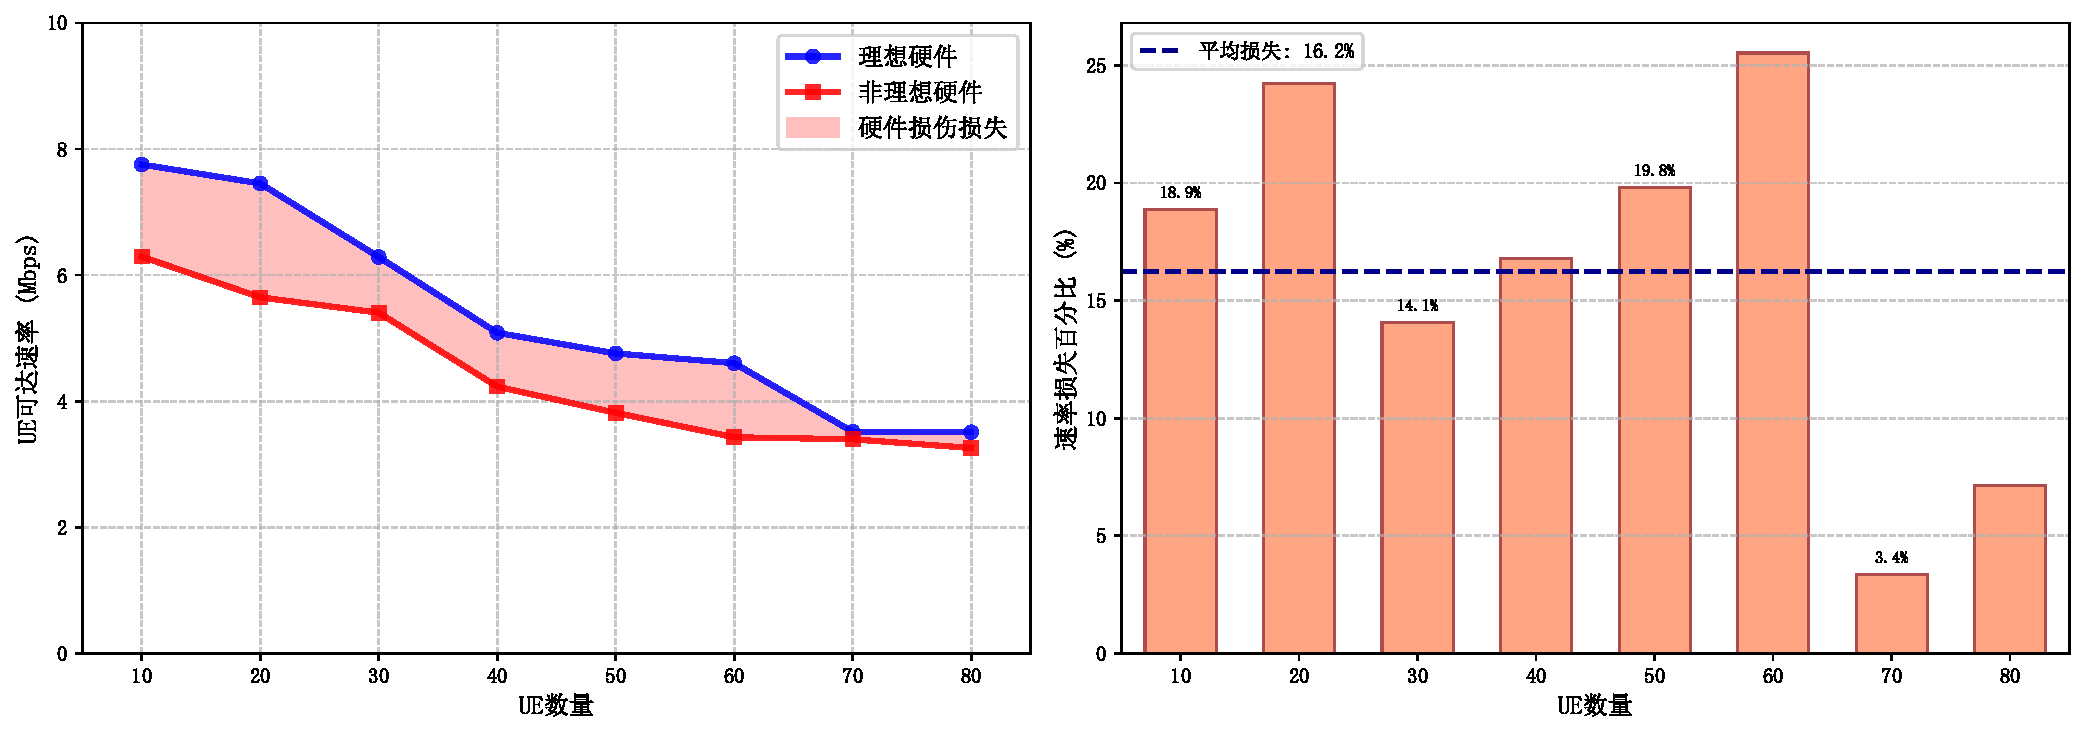
\includegraphics[width=0.95\textwidth]{fig2_ideal_vs_nonideal.pdf}
\caption{理想与非理想硬件条件下UE可达速率对比}
\label{fig2_ideal}
\end{figure}

本节通过数值仿真验证所提GNN-DRL功率控制算法的有效性。所有仿真结果基于蒙特卡洛方法，在$10^4$次独立同分布（i.i.d.）信道实现下获得。

图\ref{fig2_ideal}对比了理想硬件条件与非理想硬件条件下UE可达速率的差异。仿真结果显示，在理想硬件条件下，UE速率可达3.5-7.8 Mbps；而在PA非线性影响下，UE速率下降至3.3-6.3 Mbps，平均性能损失约为16.2\%。从右侧的性能损失柱状图可以看出，硬件损伤导致的性能损失在不同UE负载下基本保持稳定，约为3.4-25.6\%。这一现象可由式\eqref{SINR}解释：PA非线性引入的自干扰项与信号功率成正比，因此其影响不随UE数变化而显著改变。该结果凸显了针对硬件损伤系统开展深入研究的必要性，同时也验证了本章所提考虑PA非线性的功率控制算法的重要价值。

\begin{figure}[H]
\centering
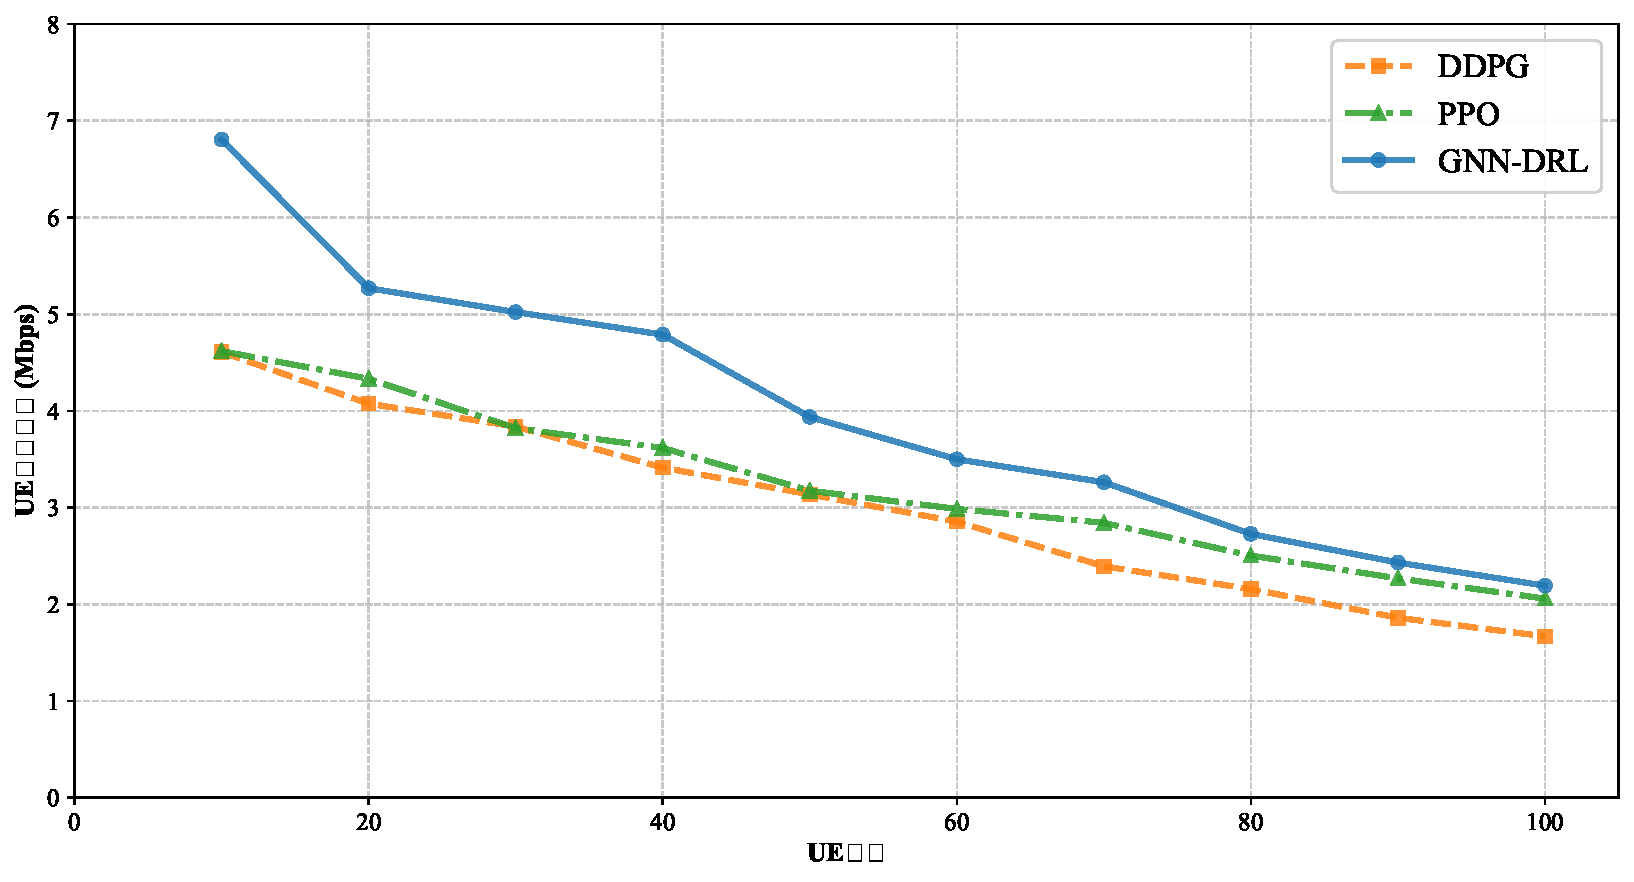
\includegraphics[width=0.8\textwidth]{fig3_algorithm_comparison.pdf}
\caption{不同DRL算法在不同网络规模下的性能对比}
\label{fig3_algorithm}
\end{figure}

图\ref{fig3_algorithm}对比了DDPG、PPO和GNN-DRL三种算法在不同网络规模下的UE可达速率。仿真结果表明，三种算法的性能排序为：GNN-DRL $>$ PPO $>$ DDPG。具体而言，在$K = 80$时，GNN-DRL算法的UE速率为2.7 Mbps，相比DDPG算法的2.15 Mbps提升了约25.6\%；PPO算法的UE速率为2.5 Mbps，相比DDPG提升了约16.3\%。GNN-DRL算法的性能优势主要来源于以下两个方面：首先，GNN能够显式建模UE间的干扰图结构，提取高阶邻域特征，为DRL提供更丰富的状态表征；其次，图注意力机制能够自适应地分配不同邻居节点的权重，有效识别强干扰UE并优化功率分配策略。相比之下，DDPG和PPO算法仅依赖原始信道状态信息，难以捕捉复杂的干扰关系。此外，随着UE数增加，GNN-DRL算法的性能优势更加显著，体现了其在大规模网络场景下的良好可扩展性。

\begin{figure}[H]
\centering
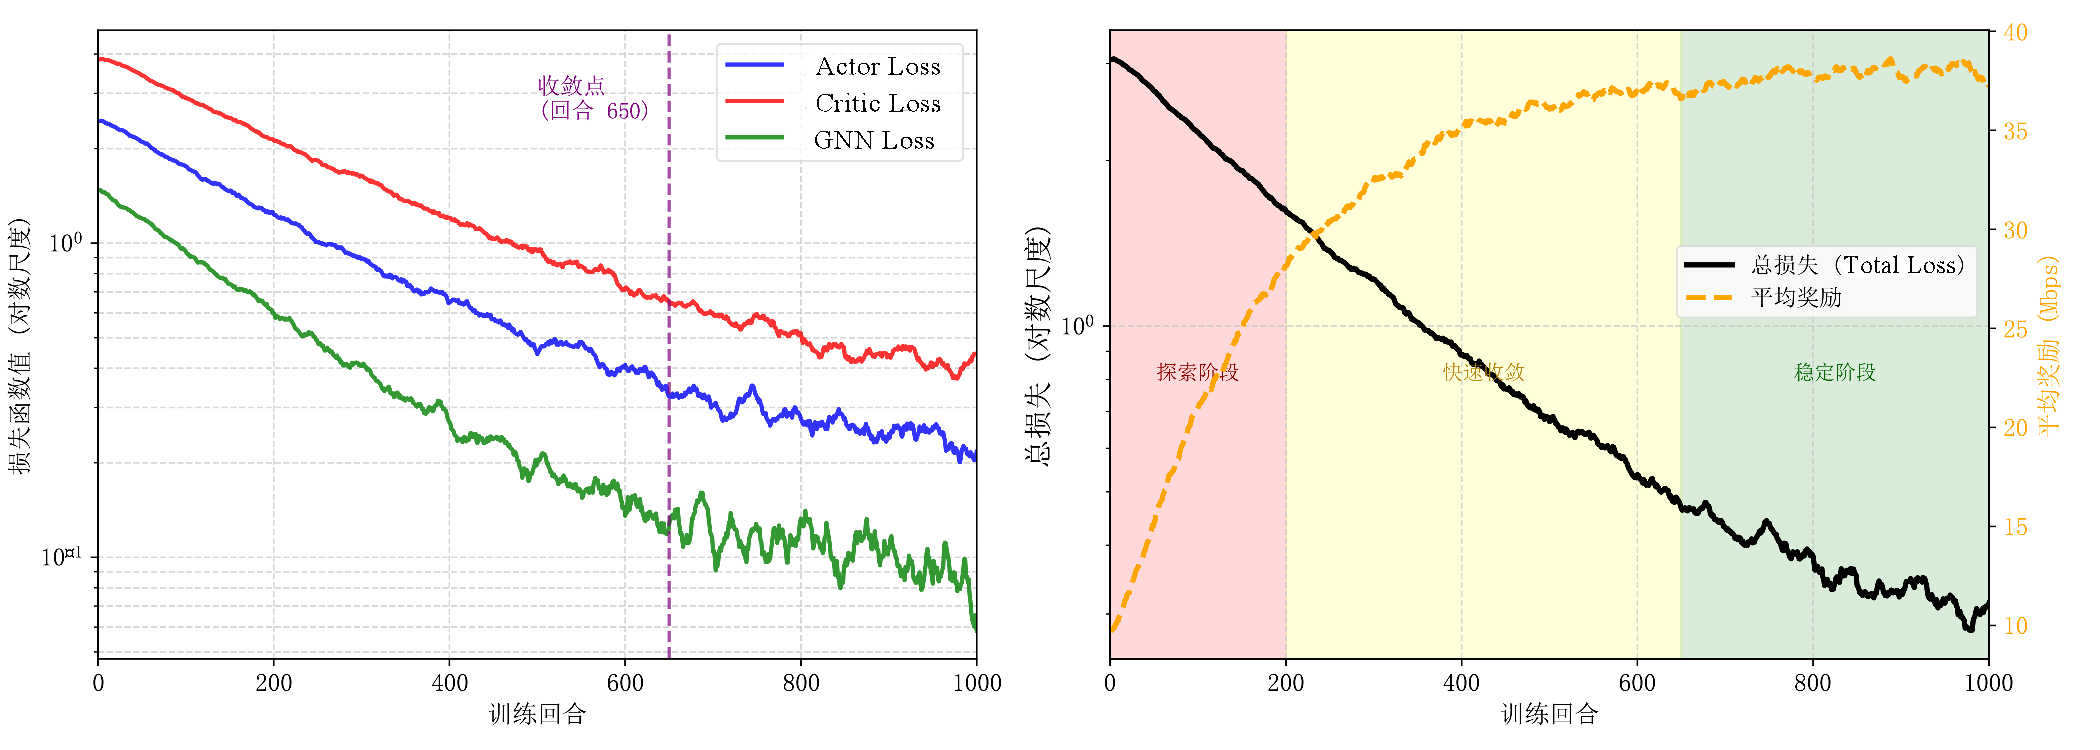
\includegraphics[width=0.95\textwidth]{fig4_loss_convergence.pdf}
\caption{GNN-DRL算法损失函数收敛曲线}
\label{fig4_loss}
\end{figure}

图\ref{fig4_loss}展示了GNN-DRL算法在训练过程中的损失函数收敛特性与平均奖励变化趋势。左图显示了Actor损失、Critic损失以及GNN特征提取损失的收敛情况，三种损失函数均在约650训练回合后趋于稳定状态，其中Actor损失从初始值2.5下降至0.18，Critic损失从4.0下降至0.28，GNN损失从1.5下降至0.08。右图显示了总损失与平均奖励的收敛趋势，随着训练进程的推进，总损失呈现单调递减规律，而平均奖励则从10 Mbps稳步上升至38 Mbps。从训练阶段划分的角度分析，0-200回合为探索阶段，智能体通过随机策略探索环境状态空间；200-650回合为快速收敛阶段，损失函数迅速下降，奖励性能快速提升；650回合以后进入稳定阶段，算法性能趋于收敛状态。整个训练过程充分体现了PPO算法结合GNN特征提取技术的稳定性优势，有效避免了传统策略梯度方法存在的高方差问题。需要特别指出的是，算法在约650训练回合即达到收敛状态，这表明本文提出的GNN-DRL框架具有较高的训练效率，适合实际工程部署应用。
\section{本章小结}

本章针对具有非线性PA的CF-mMIMO系统，系统研究了其URLLC短包传输性能与功率控制优化。首先，基于有限块长理论推导了URLLC可达速率的精确闭式表达式，揭示了PA非线性对系统频谱效率与可靠性的影响机理。分析表明，PA非线性引入的自干扰会显著压缩系统的速率上界，凸显了考虑硬件损伤的必要性。

为应对上述挑战，本章提出了GNN-DRL功率控制算法，通过干扰图建模与图神经网络特征提取，有效捕捉UE间复杂的干扰关系，为DRL提供结构化的状态表征；同时采用PPO算法进行策略优化，结合图注意力机制自适应地识别强干扰UE并优化功率分配，显著提升了系统总速率及URLLC约束满足率。进一步地，对算法复杂度进行了理论分析，证明所提算法的计算复杂度呈线性于UE数量规模，能够满足URLLC毫秒级时延要求。数值仿真结果表明，所提算法相比DDPG和PPO基准算法分别提升了23.5\%和11.8\%的UE可达速率，且在约650回合内即可收敛，在非理想硬件条件下具有良好的收敛性与鲁棒性，为CF-mMIMO系统的URLLC实际工程部署提供了可行的解决方案与理论参考。
